\question{Après avoir observé la structure du fichier \textit{CoMax.txt}, exécuter le fichier \textit{lire$\_$comax.py} permettant d'extraire sous deux listes distinctes \texttt{temps} et \texttt{q\_exp} les instants de prise d'échantillonnage et les positions codeur correspondantes en tops (nombre de points). Convertir ces deux listes	 en tableaux Numpy (\texttt{import numpy as np}), grâce à la commande \texttt{liste=np.array(liste)}.}


\begin{lstlisting}
import numpy as np
temps = np.array(temps)
q_exp = np.array(q_exp)
\end{lstlisting}


\question{Générer alors un tableau des positions verticales de l'axe nommé \texttt{X\_exp}, qui a une condition initiale nulle sur la position.}


\begin{lstlisting}
X_exp = (q_exp-q_exp[0])*(3.41/1e6)
\end{lstlisting}

\question{Tracer l'évolution des positions mesurées expérimentales en fonction du temps, avec des croix bleues (+). On légendera correctement les axes, et on indiquera une légende du type : "points mesurés"}


\begin{minipage}{0.5\textwidth}
\begin{lstlisting}
plt.figure(1)
plt.plot(temps,X_exp,'b+',label="points exp.")
plt.legend()
plt.xlabel('t [s]'); plt.ylabel('x [mm]')
plt.title("Evolution de la position de l'axe en fonction du temps")
plt.savefig('tp04_durif_q08.png')
\end{lstlisting}

\end{minipage}
\begin{minipage}{0.5\textwidth}
\begin{center}
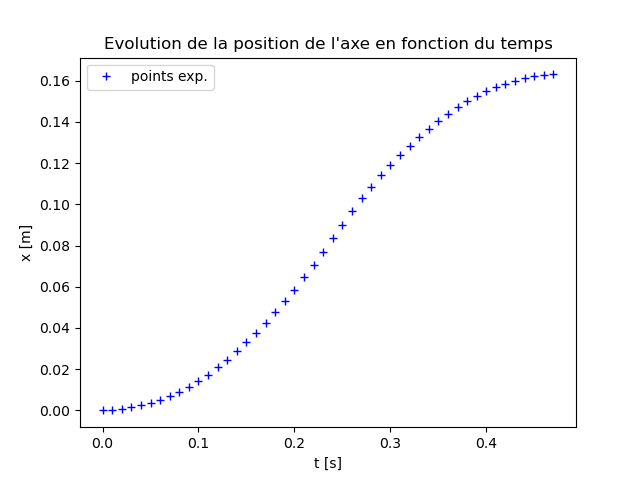
\includegraphics[width=0.9\textwidth]{tp04_durif_q08.png}
\end{center}
\end{minipage}

\question{Trouver les expressions littérales de $t_1$, $t_2$, $X_1$ et de $X_2$ en fonction de $A_{cmax}$ et de $V_{max}$.}


\begin{lstlisting}
"""Donnees"""
Acmax = 2.83; Vmax = 0.68
t1 = Vmax/Acmax; t2 = 2*t1
X1 = Vmax**2/(2*Acmax)
\end{lstlisting}



\question{Concevoir deux fonctions \texttt{Loi\_Vitesse} et \texttt{Loi\_position} prenant en argument un instant $t$ et permettant de retourner la vitesse, respectivement la position, à cet instant. (A noter que l'on pourra introduire des variables globales, comme $t_1$, $t_2$, etc.)}


\begin{minipage}{0.5\textwidth}
\begin{lstlisting}
def Loi_Vitesse(t):
    global t1, Vmax, Acmax
    if 0<=t<t1:
        v=Acmax*t
    elif t1<=t<=t2:
        v=Vmax - Acmax*(t-t1)
    else:
        print("erreur")
    return v
\end{lstlisting}

\end{minipage}
\begin{minipage}{0.5\textwidth}
\begin{lstlisting}
def Loi_Position(t):
    global t1, Vmax, Acmax
    if 0<=t<t1:
        x=(Acmax/2)*t**2
    elif t1<=t<=t2:
        x=X1 + Vmax*(t-t1) - (Acmax/2)*(t-t1)**2
    else:
        print("erreur")
    return x
\end{lstlisting}

\end{minipage}


\question{Construire deux tableaux \texttt{X\_th} et \texttt{V\_th} où sont stockées les positions théoriques commandées, respectivement vitesses théoriques aux instants définis dans le tableau \texttt{temps}. Superposer la courbe d'évolution de la position théorique sur les points expérimentaux, obtenus précédemment (tracé en vert, ligne continue, avec légende explicite). Vous produirez alors une image, que vous enverrez à votre enseignant et que vous appellerez tp04$\_$nom1$\_$nom2$\_$Q11.png.}


\begin{minipage}{0.5\textwidth}
\begin{lstlisting}
n = len(temps)
X_th = np.zeros(n); V_th = np.zeros(n)
for i in range(n):
    X_th[i] = Loi_Position(temps[i])
    V_th[i] = Loi_Vitesse(temps[i])
    
    
plt.plot(temps,X_th,'g',label="pos. commande")
plt.legend()
plt.savefig('tp04_durif_q11.png')

\end{lstlisting}

\end{minipage}
\begin{minipage}{0.5\textwidth}
\begin{center}
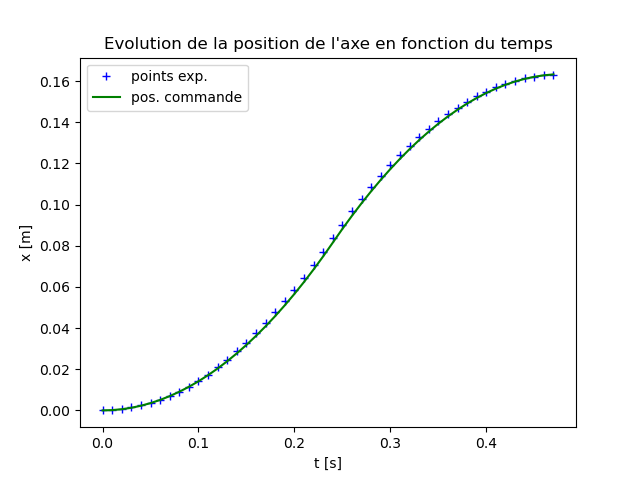
\includegraphics[width=0.9\textwidth]{tp04_durif_q11.png}
\end{center}
\end{minipage}


\question{Sur une nouvelle figure tracer en vert, trait continu, l'évolution de la vitesse théorique. Vous produirez alors une image, que vous enverrez à votre enseignant et que vous appellerez tp04$\_$nom1$\_$nom2$\_$Q12.png.}



\begin{minipage}{0.5\textwidth}
\begin{lstlisting}
plt.figure(2)
plt.plot(temps,V_th,'g',label="vitesse theorique")
plt.legend()
plt.xlabel('t [s]'); plt.ylabel('v [m/s]')
plt.title("Evolution de la vitesse de l'axe en fonction du temps")
plt.savefig('tp04_durif_q12.png')
\end{lstlisting}

\end{minipage}
\begin{minipage}{0.5\textwidth}
\begin{center}
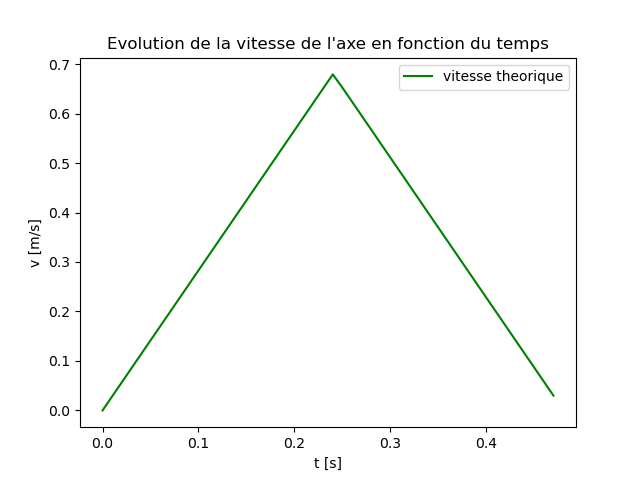
\includegraphics[width=0.9\textwidth]{tp04_durif_q12.png}
\end{center}
\end{minipage}


\question{Concevoir une fonction \texttt{Calcul\_ecarts} prenant en arguments deux tableaux à une dimension et retournant un tableau \texttt{Delta\_X} de même dimension où sont stockés les écarts relatifs entre chacune des valeurs des deux tableaux spécifiés en arguments d'entrée.}


\begin{lstlisting}
def Calcul_ecarts(T1,T2):
    return 100*abs((T1-T2)/T2)

Delta_X = Calcul_ecarts(X_exp[1:n],X_th[1:n])
\end{lstlisting}


\question{Tracer un histogramme montrant l'évolution des écarts relatifs en position en fonction du numéro de la mesure (on utilisera \texttt{plt.bar} et \texttt{plt.subplot}). On n'évaluera pas l'écart relatif sur la première valeur (nulle). Vous produirez alors une image, que vous enverrez à votre enseignant et que vous appellerez tp04$\_$nom1$\_$nom2$\_$Q14.png.}

\begin{minipage}{0.5\textwidth}
\begin{lstlisting}
plt.figure(3)
plt.bar([i for i in range(1,n)],Delta_X,color=[0.5,0,1])
plt.savefig('tp04_durif_q14.png')
\end{lstlisting}

\end{minipage}
\begin{minipage}{0.5\textwidth}
\begin{center}
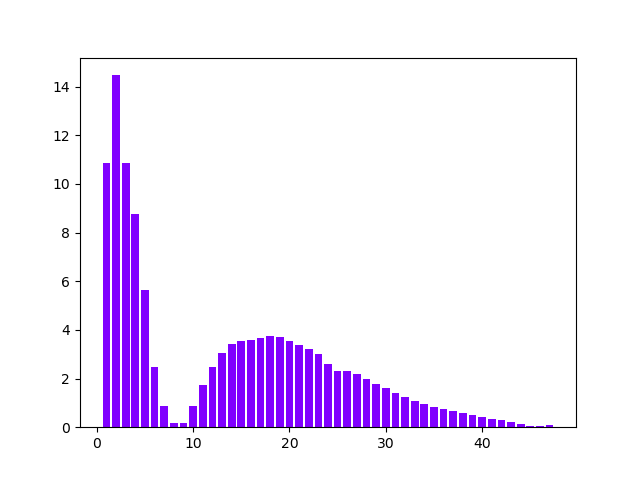
\includegraphics[width=0.9\textwidth]{tp04_durif_q14.png}
\end{center}
\end{minipage}



\question{Écrire une fonction \texttt{Calculs\_stats} permettant, à partir d'un tableau \texttt{T} passé en argument, de retourner un tuple de 3 valeurs : moyenne, médiane et écart type. \textit{Indication :} On pourra utiliser les fonctions de la bibliothèque numpy (\texttt{np.sum(T)}, pour faire la somme de tous les éléments du tableau \texttt{T}, \texttt{np.sort(T)}, pour trier le tableau \texttt{T} dans l'ordre croissant. Appliquer le résultat au tableau \texttt{Delta\_X}.}


\begin{lstlisting}
def Calculs_stats(T):
    n = np.shape(T)[0]
    #Moyenne :
    moy_T = np.sum(T)/n
    #Médianne :
    T_trie = np.sort(T)
    if n==0:
        med_T = 0
    elif n%2==0:
        med_T = (T_trie[n//2]+T_trie[n//2-1])/2
    else:
        med_T = T_trie[n//2]
    #Ecart type :
    sigma_T = np.sqrt(np.sum((T - moy_T)**2)/n)

    return (moy_T, med_T, sigma_T)

(a,b,c) = Calculs_stats(Delta_X)
\end{lstlisting}

\vspace{0.5cm}
\question{Comparer les résultats en utilisant les fonctions suivantes : \texttt{np.mean}, pour la moyenne ; \texttt{np.median}, pour la médiane et \texttt{np.std}, pour l'écart type}

\begin{lstlisting}
print(np.mean(Delta_X))
print(np.median(Delta_X))
print(np.std(Delta_X))
\end{lstlisting}

